\chapter{ Analyse et Sp\'{e}cifications besoins }
\section{Introduction}


Cette partie consiste en une \'{e}tape analytique dans laquelle nous allons
recenser et factoriser les besoins des utilisateurs de l'application. Ceci est
fortement li\'{e} \`{a} l'\'{e}tude pr\'{e}alable men\'{e}e au
Cours du premier chapitre.
Pour ce faire cette phase doit r\'{e}pondre aux questions suivantes :
Quels sont les besoins fonctionnels de l'application ?
Quelles sont les contraintes qui doivent \^{e}tre prises en consid\'{e}ration?

   \section{ Les acteurs du syst\`{e}me }
C'est une entit\'{e} externe qui agit sur le syst\`{e}me (op\'{e}rateur, autre syst\`{e}me,
\ldots{}).Il peut consulter
Ou modifier l'\'{e}tat du syst\`{e}me.
En r\'{e}ponse \`{a} l'action d'un acteur, le syst\`{e}me fournit un service qui
correspond \`{a} son besoin.
Le principal acteur de syst\`{e}me :
\begin{itemize}
\item{  \textbf{L'administrateur :} entit\'{e} externe principale. Son r\^{o}le est qui a le droit de
g\'{e}rer un projet (cr\'{e}er, modifier, supprimer).
Aussi son r\^{o}le et de g\'{e}rer l'affectation des taches aux membres
correspondants.
}

\item{ \textbf{Le membre : } entit\'{e} externe secondaire, il peut se connecter pour consulter la
t\^{a}che en cours que l'administrateur lui a effectu\'{e} et la marquer comme
termin\'{e}e ou non.
}
\end{itemize}

Ce tableur pr\'{e}sente les roles selon les acteurs:

\begin{table}[H]
\centering
\begin{tabular}{|l|l|l|}
\hline
                                            & Administrateur & Membre  \\
\hline
Authentification~                           & X              & X       \\
\hline
Création d’un projet                        & X              &         \\
\hline
Ajout d’une tache                           & X              & X       \\
\hline
Modifier l’état d’une tâche                 & X              &         \\
\hline
Ajout d’un client/membre                    & X              &         \\
\hline
Consultation des rapports                   & X              &         \\
\hline
Consulter la carte géographique des clients & X              & X       \\
\hline
\end{tabular}
\centering
\caption{Rôles  des acteurs.}
\end{table}


\section{ Sp\'{e}cifications besoins}

  \subsection{Besoins fonctionnels}

Le besoin primordiale de notre application et de permettre à l’administrateur
de « Cherchini » de gérer les projets et ceci consiste à :

\subsubsection{G\'{e}rer les projets}

\begin{itemize}
\item{La cr\'{e}ation d’un projet.}
\item{La modification d'un projet.}
\item{La suppression d'un projet.}
\item{Consulter les projets et les t\^{a}che et les d\'{e}tails correspondants.}
\item{Affecter les membres correspondants \`{a} chaque projet.}
\end{itemize}

\subsubsection{G\'{e}rer les t\^{a}che}

\begin{itemize}
\item{La cr\'{e}ation d'une t\^{a}che.}
\item{La modification d'une t\^{a}che.}
\item{La suppression d'une t\^{a}che.}
\item{Consulter les t\^{a}che et les d\'{e}tails correspondants.}
\item{Affecter le membre correspondant \`{a} chaque t\^{a}che.}
\end{itemize}

\subsubsection{G\'{e}rer les membres}

\begin{itemize}
\item{La cr\'{e}ation d'un membre.}
\item{La modification d'un membre.}
\item{La suppression d'un membre.}
\item{Consulter les membres et leurs d\'{e}tails correspondants.}
\item{Affecter les membres correspondants \`{a} chaque projet.}
\end{itemize}

\subsubsection{G\'{e}rer les clients}

\begin{itemize}
\item{La cr\'{e}ation d'un .}
\item{La modification d'un client.}
\item{La suppression d'un client.}
\item{Consulter les clients et leurs d\'{e}tails correspondants.}
\end{itemize}

\subsubsection{
Suivre le d\'{e}roulement des projets}

\begin{itemize}
\item{ Suivre le travail des \'{e}quipes en consultant le diagramme Gantt pour chaque projet.}
\item{Consulter les rapports des co\^{u}ts et les dur\'{e}es selon les projets et les clients   .}
\item{Consulter la carte g\'{e}ographique des g\'{e}olocalisations des  .}
\end{itemize}

  \subsection{Besoins non fonctionnels}
Les besoins non fonctionnels sp\'{e}cifient les propri\'{e}t\'{e}s du syst\`{e}me afin de
garantir la Coh\'{e}rence, la confidentialit\'{e} et l'int\'{e}grit\'{e} des donn\'{e}es.
Le syst\`{e}me doit \^{e}tre fiable: la validit\'{e} de l`application.
R\'{e}utilisabilit\'{e}: aptitude de site \`{a} \^{e}tre utilis\'{e} en tout ou en partie dans de
nouvelles applications.

\subsubsection{La performance d'ex\'{e}cution}

Le temps d'ex\'{e}cution du syst\`{e}me doit \^{e}tre minimal pour ne pas g\^{e}ner
l'utilisateur. Ce temps d\'{e}pend de la complexit\'{e} du code impl\'{e}ment\'{e}, du
serveur d'application utilis\'{e}, du d\'{e}bit de la ligne de connexion et de la
conception de la base de donn\'{e}es.

\subsubsection{La s\'{e}curit\'{e}}

Le syst\`{e}me doit respecter un niveau de s\'{e}curit\'{e} \'{e}lev\'{e} afin de garantir la
confidentialit\'{e} de l'acc\`{e}s des membres

\subsubsection{L'ergonomie }

L'interface de cette application doit \^{e}tre ergonome, conviviale et voire m\^{e}me
apte \`{a} aider l'utilisateur \`{a} mieux g\'{e}rer son espace de travail.


\section{ Diagramme de cas d'utilisation g\'{e}n\'{e}rale }
Le diagramme de cas d'utilisation permet de d\'{e}crire l'interaction entre
l'acteur et le syst\`{e}me.
Le cas d'utilisation est une description des interactions qui vont permettre \`{a}
l'acteur d'atteindre son objectif en utilisant le syst\`{e}me. Un acteur et un cas
d'utilisation sont mis en relation par une association repr\'{e}sent\'{e}e par une
ligne.
Le but principal du diagramme du cas d'utilisation est de d\'{e}finir le syst\`{e}me
du point de vue des utilisateurs et de d\'{e}finir les limites pr\'{e}cises du syst\`{e}me en
utilisant une notation tr\`{e}s simple






\FloatBarrier
\begin{figure}[H]
\center
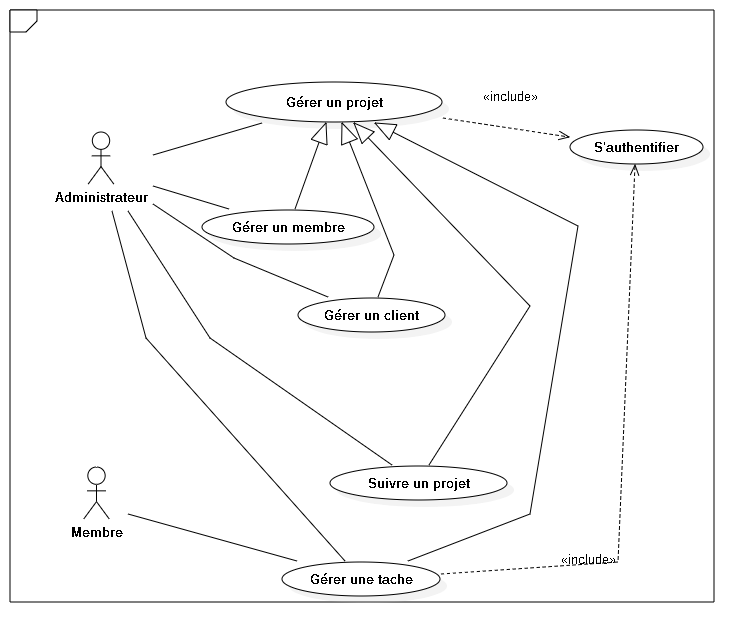
\includegraphics[width=13cm,height=10cm]{./figures/ucG.png}
\caption{Diagramme de cas d'utilisation g\'{e}n\'{e}rale.}

\end{figure}
\FloatBarrier







\section{Backlog de planning}

Apr\'{e}s avoir d\'{e}finit les acteurs des systémes et les diff\'{e}rentes interactions nous pouvons maintenant définir notre Product Backlog
puis nous pr\'{e}cisions la planification des sprints.

\subsection{Les fonctionnalit\'{e}s du Backlog}
Le Backlog est un art\'{e}fact tr\`{e}s important dans SCRUM. C'est l'ensemble des caract\'{e}ristiques
fonctionnelles ou techniques qui constituent le produit souhait\'{e}.
Nous allons les d\'{e}crire en d\'{e}tails dans le tableau qui suit :



\begin{table}

\begin{tabular}{|l|l|l|}
\hline
Fonctionnalité                                                                                              & Acteur                          & Description                                                                                                                                                     \\
\hline
Gérer un projet                                                                                             & Administrateur                  & \begin{tabular}[c]{@{}l@{}}L’administrateur peut gérer un projet et ses \\tâches correspondantes d’affectation\end{tabular}                                     \\
\hline
Mettre à jour un                                                                                            & \multirow{3}{*}{Administrateur} & \multirow{3}{*}{\begin{tabular}[c]{@{}l@{}}L’administrateur peut changer les détails \\du projet ainsi que l’affectation des membres\\~au projet\end{tabular}}  \\
\cline{1-1}
Projet                                                                                                      &                                 &                                                                                                                                                                 \\
\cline{1-1}
                                                                                                            &                                 &                                                                                                                                                                 \\
\hline
\begin{tabular}[c]{@{}l@{}}Créer ,Modifier ,\\Supprimer un membre\end{tabular}                              & Administrateur                  & \begin{tabular}[c]{@{}l@{}}L’administrateur peut manipuler les données \\des membres\end{tabular}                                                               \\
\hline
\begin{tabular}[c]{@{}l@{}}Créer ,Modifier ,\\Supprimer un client\end{tabular}                              & Administrateur                  & \begin{tabular}[c]{@{}l@{}}L’administrateur peut manipuler les \\données des clients\end{tabular}                                                               \\
\hline
Consulter les rapports                                                                                      & Administrateur                  & L’administrateur peut accéder aux rapports                                                                                                                      \\
\hline
\begin{tabular}[c]{@{}l@{}}Consulter les coordonnées \\des clients sur la carte\\~géographique\end{tabular} & Administrateur                  & \begin{tabular}[c]{@{}l@{}}L’administrateur peut accéder aux \\coordonnées géographiques des clients\end{tabular}                                               \\
\hline
\begin{tabular}[c]{@{}l@{}}Changer l’état et la\\~progression approximative \\de ses tâches\end{tabular}    & Membre                          & \begin{tabular}[c]{@{}l@{}}Le membre peut changer ses taches \\courantes selon l’avancement.\end{tabular}                                                       \\
\hline
\end{tabular}
\centering
\caption{Product Backlog}
\end{table}

\newpage

\subsection{ Planification des sprints}

\FloatBarrier
\begin{table}

\begin{tabular}{|l|l|l|}
\hline
\multirow{2}{*}{Release 1} & Gestion des projets                        & 20 jours  \\
\cline{2-3}
                           & Gestion des membres                        & 7 jours   \\
\hline
\multirow{5}{*}{Release 2} & Gestion des clients                        & 2 jours   \\
\cline{2-3}
                           & Authentification                           & 5 jours   \\
\cline{2-3}
                           & Création des interfaces administrateurs    & 20 jours  \\
\cline{2-3}
                           & Création des interfaces membres            & 5 jours   \\
\cline{2-3}
                           & Modification et design des interfaces~ ~ ~ & 15 jours  \\
\hline
\multirow{2}{*}{Release 3} & Intégration des données                    & 10 jours  \\
\cline{2-3}
                           & Affichage des rapports                     & 7 jours   \\
\hline

\end{tabular}
\centering
\caption{Planification des sprints }
\end{table}
\FloatBarrier


\subsection{Diagramme de Gantt}

\FloatBarrier
\begin{figure}[H]
\center
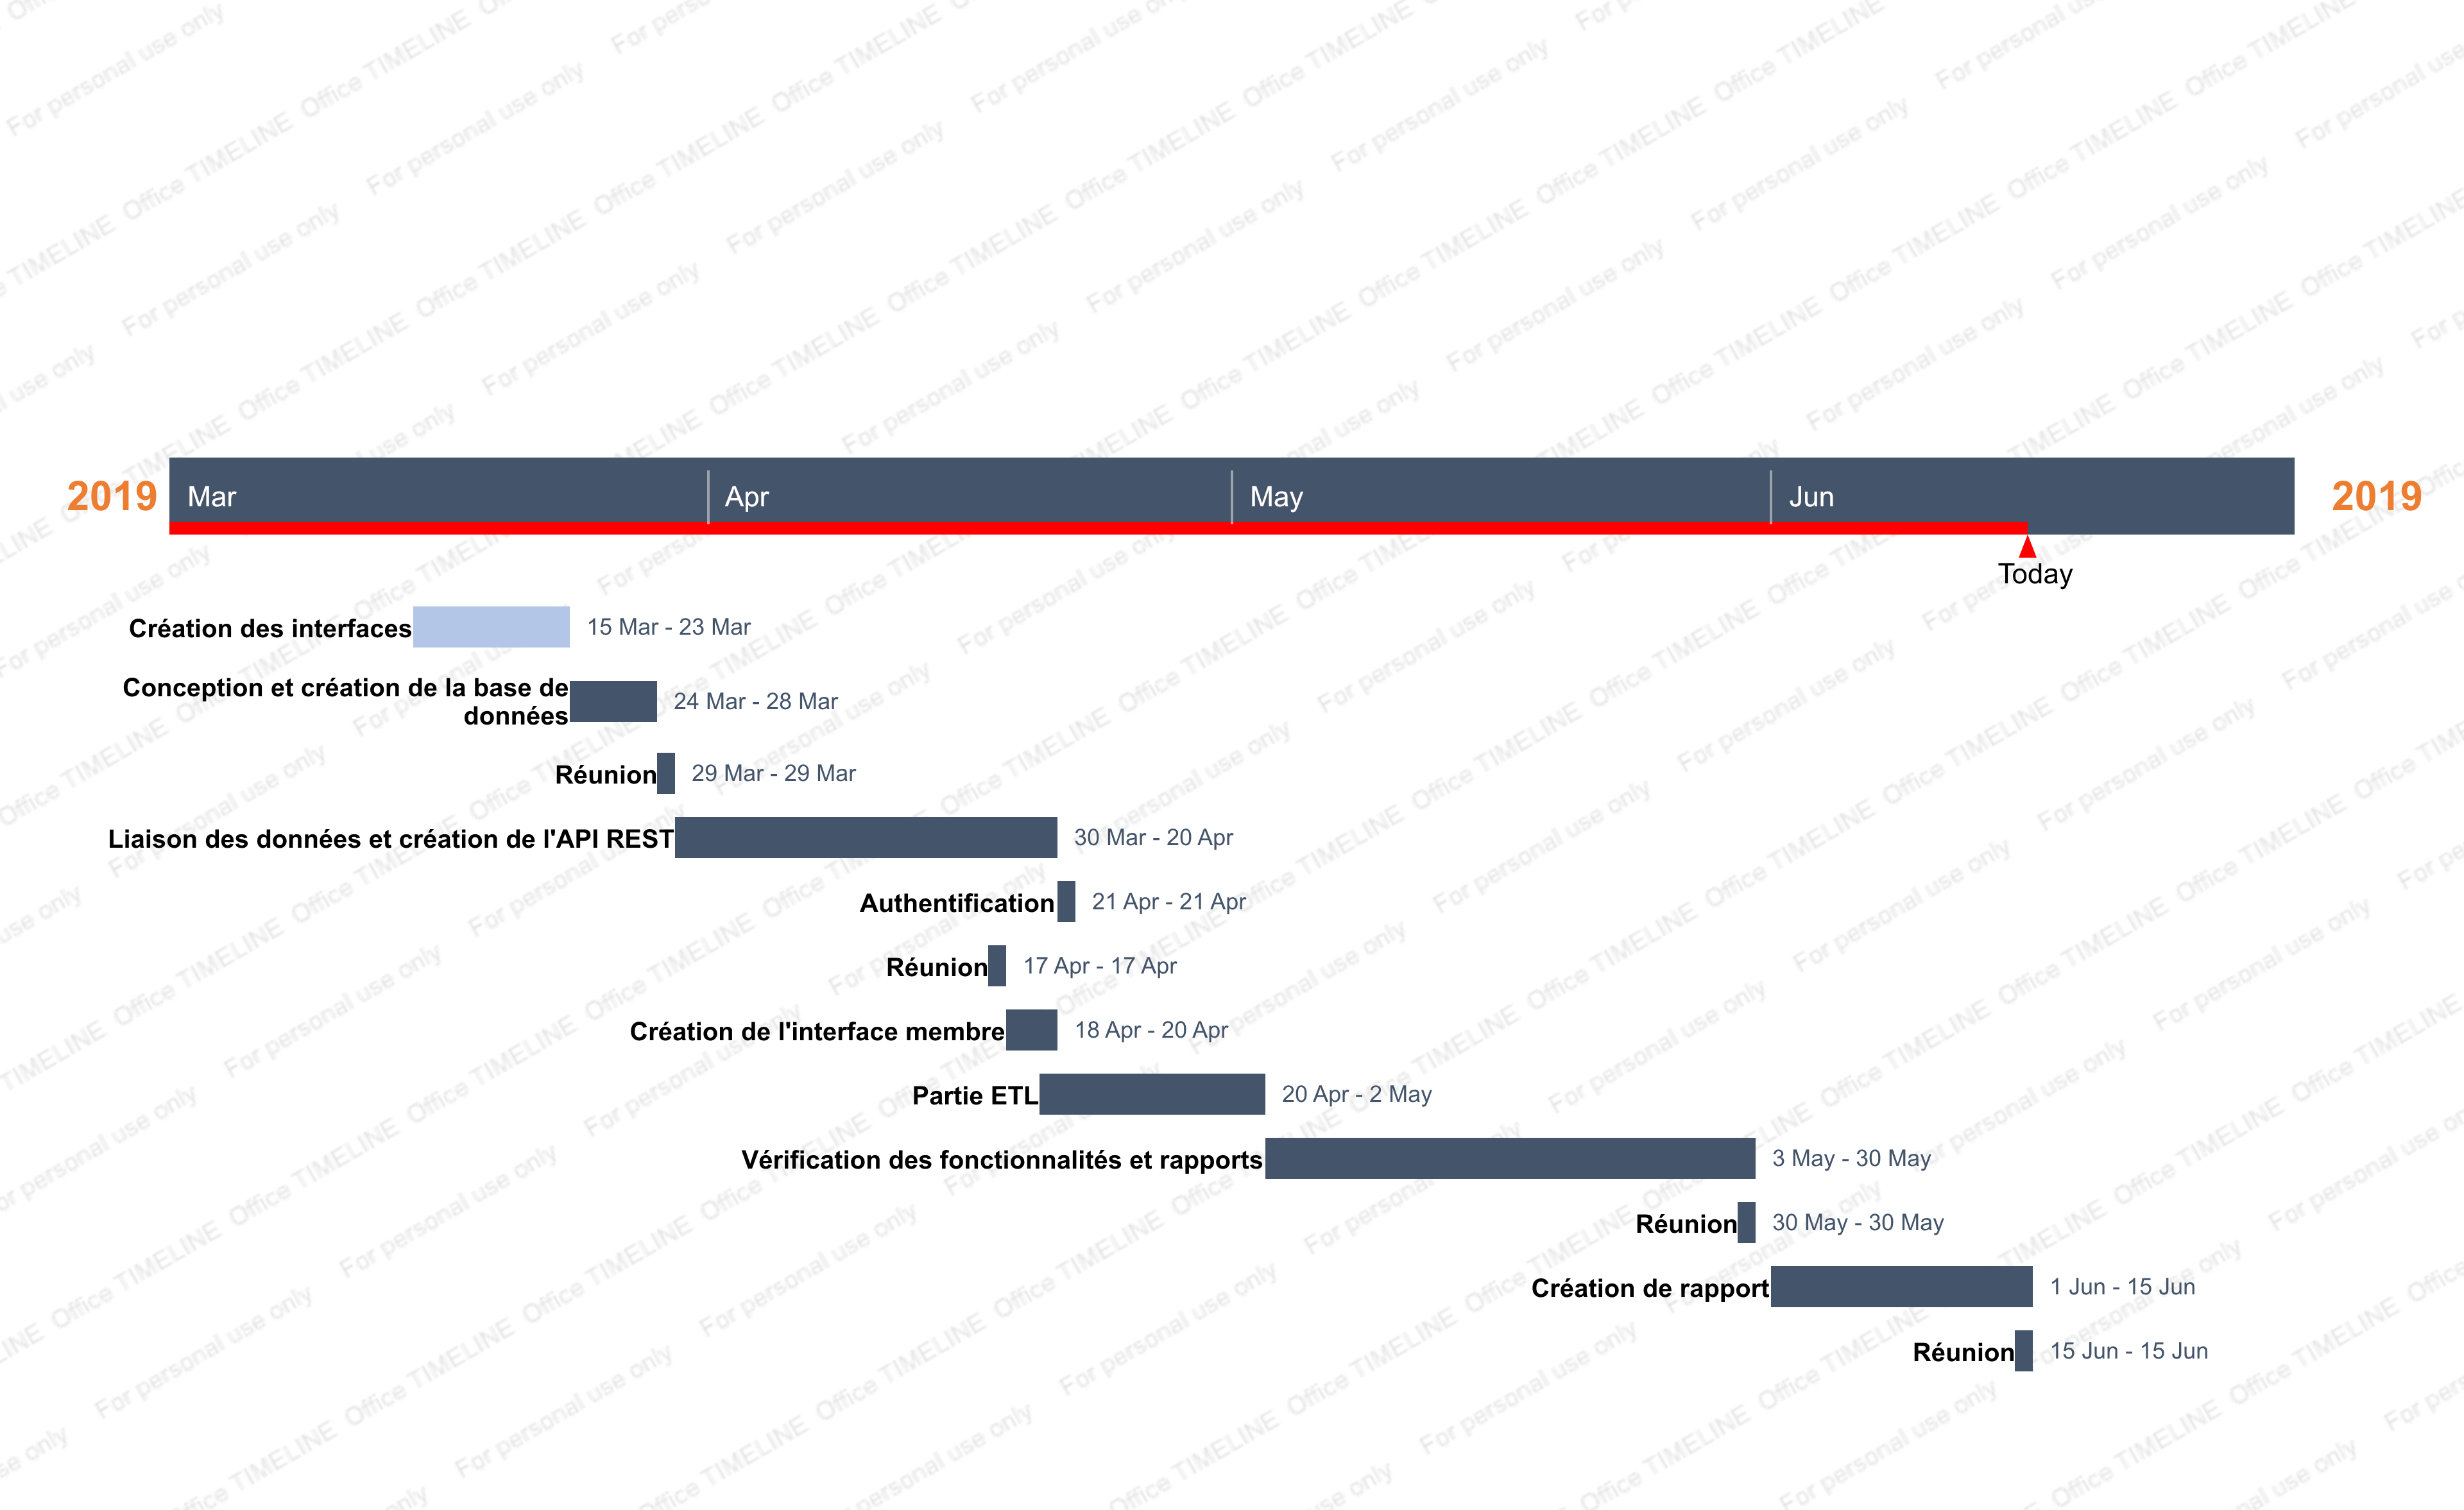
\includegraphics[width=15cm,height=15cm]{./figures/gantt.png}
\caption{Diagramme de Gantt.}
\end {figure}
\FloatBarrier

%\begin{figure}[!h]
%\center
%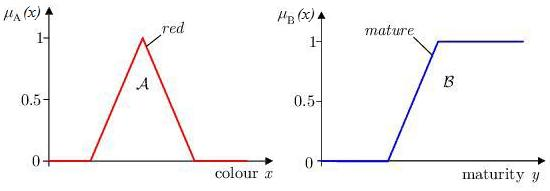
\includegraphics[width=10cm,height=6cm]{Relation.png}
%\caption{Titre de la Figure.}
%
%\end{figure}

%~~~~Bla bla bla exempe d'une liste:
%\begin{itemize}
%\item{}
%\item{}
%\item{}
%\item{}
%\end{itemize}

